\documentclass{beamer}
\usepackage{graphicx}
\title{Trusted, efficient routers using the AJIT-64 multi-core system}
\author{Madhav Desai, D. Manjunath\\
Department of Electrical Engineering\\ IIT Bombay}

\begin{document}
\maketitle

\frame[containsverbatim]{\frametitle{Overview}
\begin{itemize}
\item We have completed the design and development of a multi-core AJIT processor with
64-bit ISA extensions.
\item The multi-core processor can have
\begin{itemize}
\item Up to 4 cores.
\item Each core can have 1 or 2 execution threads.
\item Each execution thread can be either a 32-bit only thread or a 64/32-bit thread.
\end{itemize}
\item GNU bin-utils (assembler, debugger, disassembler, linker) for the 64-bit extensions have
	been implemented.
\item We propose a concept network router based on the AJIT multi-core platform.
\end{itemize}
}

\frame[containsverbatim]{\frametitle{Proposed platform: Phase 1}
\begin{figure}
  \centering
  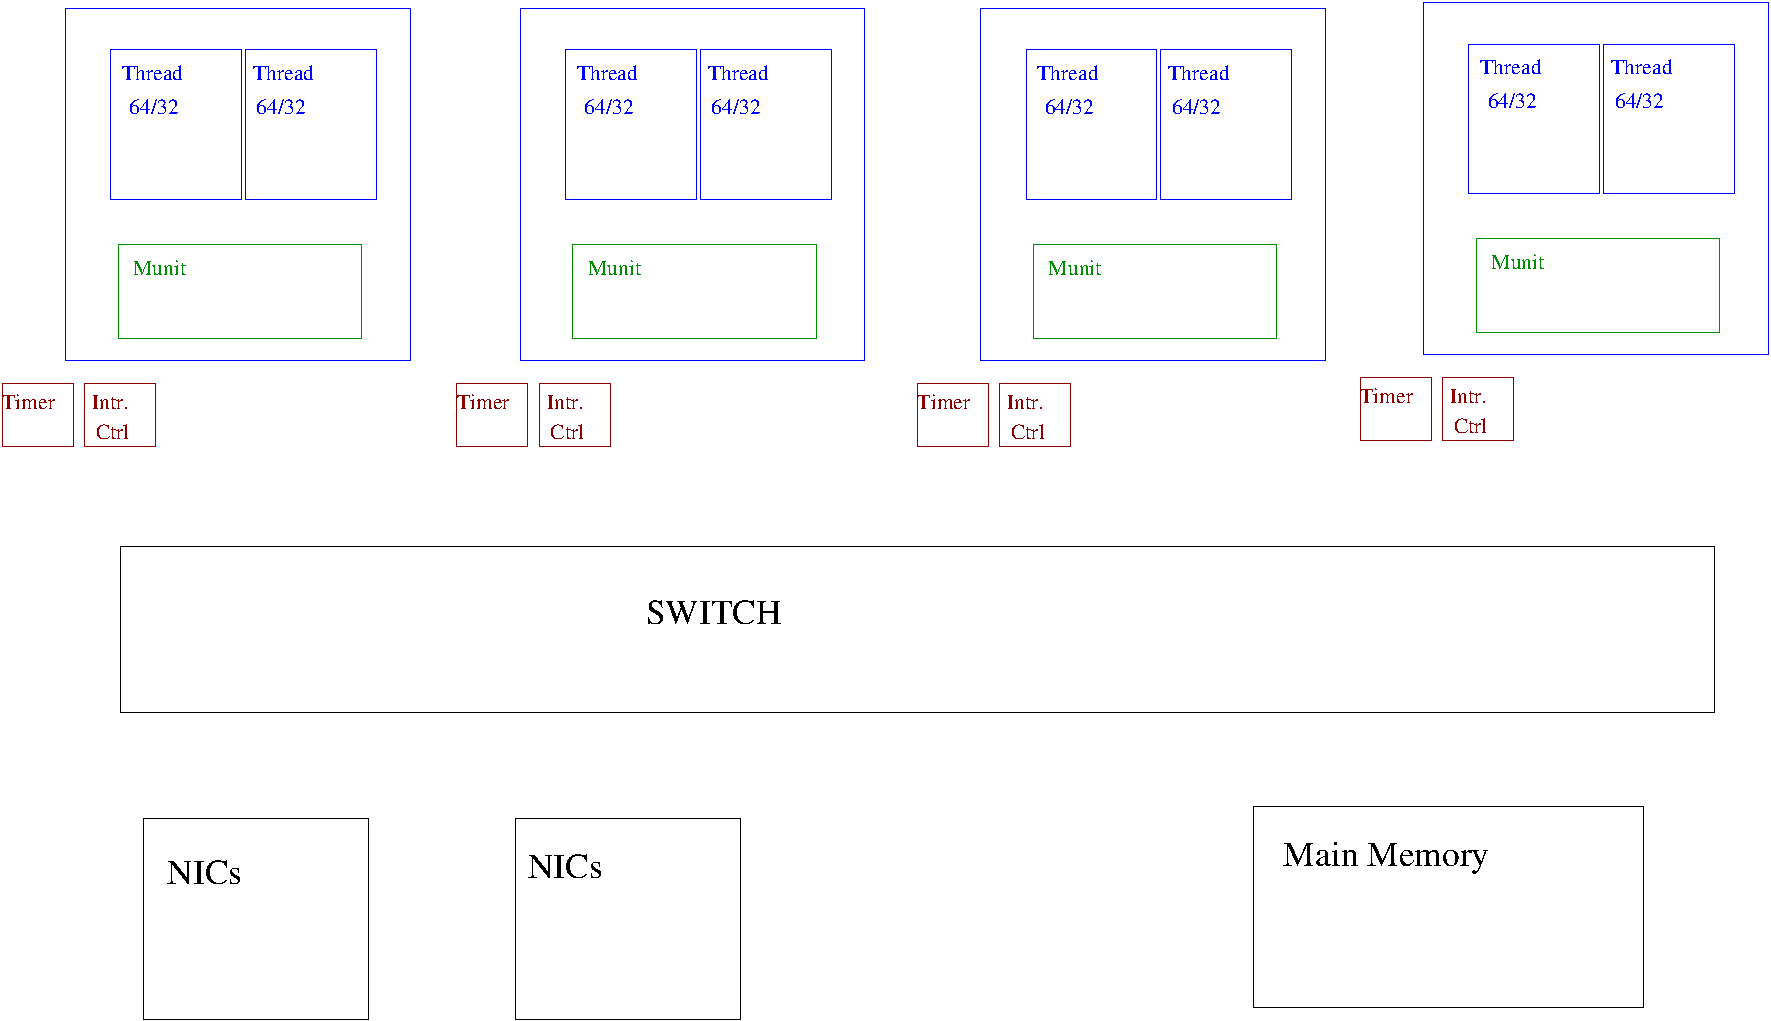
\includegraphics[width=10cm]{figs/Router_I.pdf}
  \caption{Router platform: phase 1}
\end{figure}
}

\frame[containsverbatim]{\frametitle{Comments on the proposed platform: Phase 1}
\begin{itemize}
\item Vanilla NICs.
\begin{itemize}
\item NIC and main memory communicate directly.
\item NIC to NIC direct paths are provided.
\end{itemize}
\item Processor cores handle route lookup.
\item Software optimization.
\end{itemize}
}

\frame[containsverbatim]{\frametitle{Proposed platform: Phase 2}
\begin{figure}
  \centering
  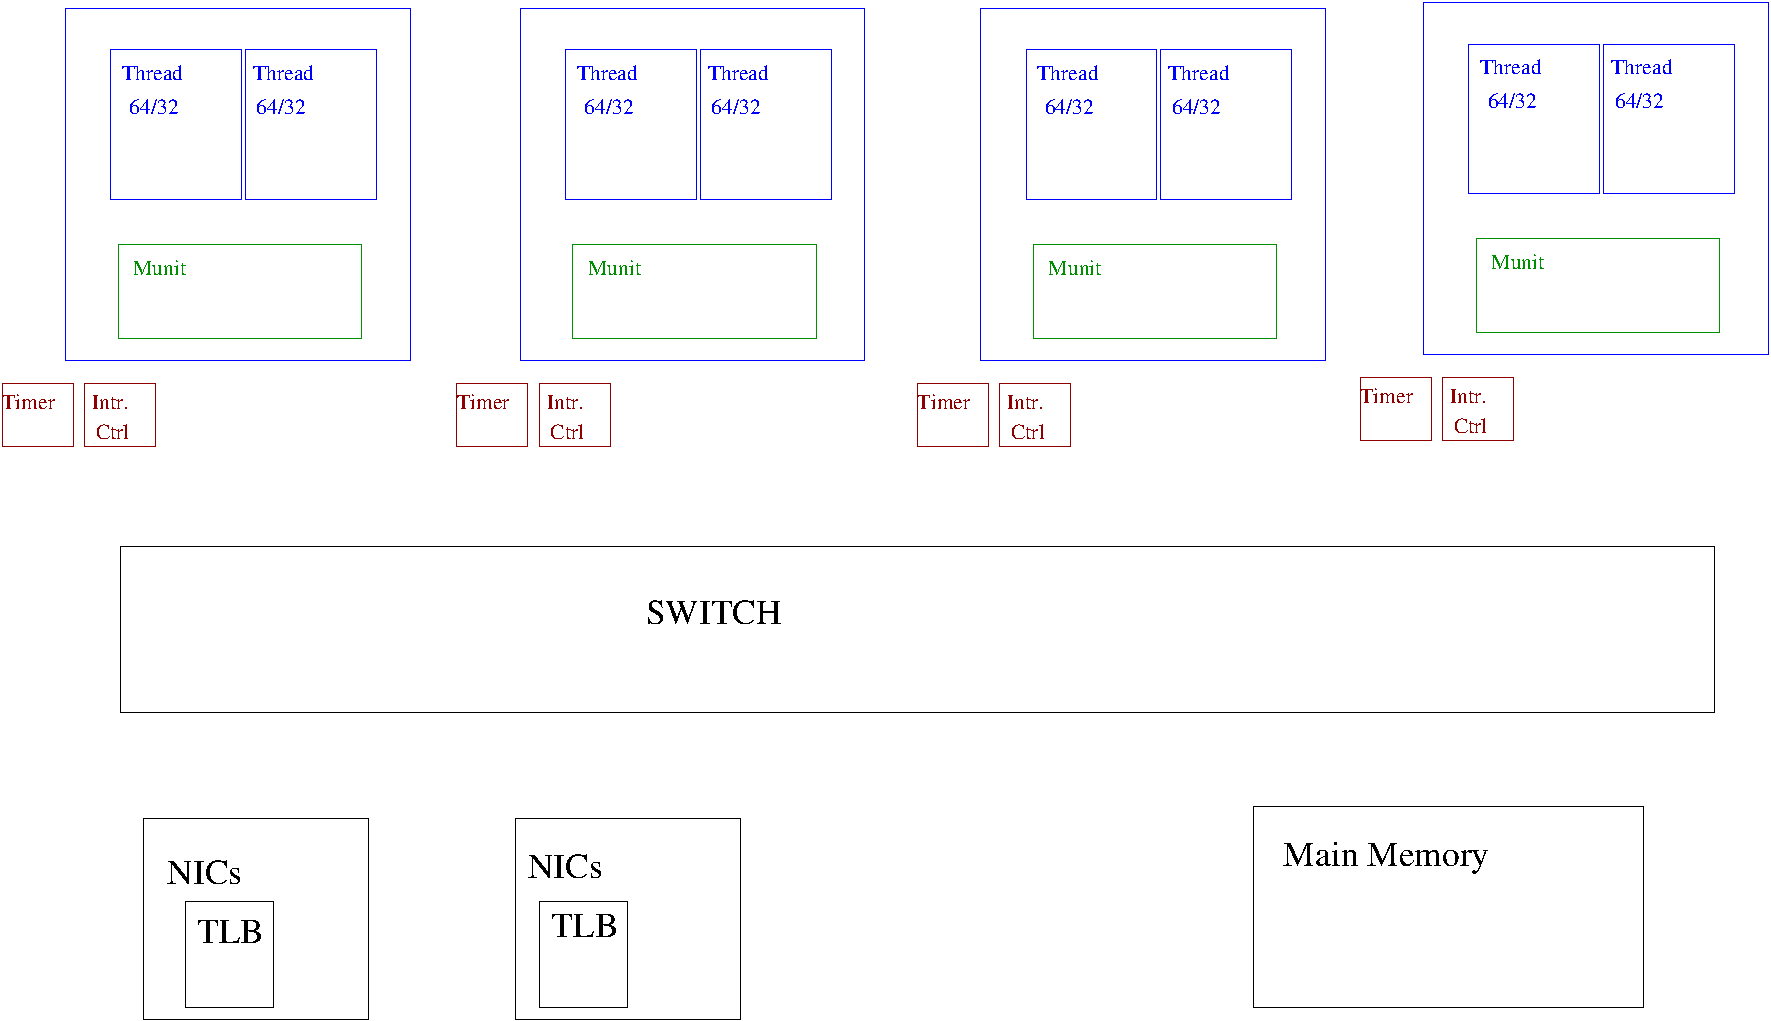
\includegraphics[width=10cm]{figs/Router_II.pdf}
  \caption{Router platform: phase 2}
\end{figure}
}

\frame[containsverbatim]{\frametitle{Comments on the proposed platform: Phase 2}
\begin{itemize}
\item NICs with lookup caches.
\begin{itemize}
\item NIC and main memory communicate directly.
\item NIC to NIC communication is possible using
common switch.
\item On lookup cache hit, NIC to NIC packet
movement.
\item Packet modification in NIC.
\end{itemize}
\item Processor cores handle non-hit route lookups.
\end{itemize}
}

\frame[containsverbatim]{\frametitle{Proposed platform: Phase 3}
\begin{figure}
  \centering
  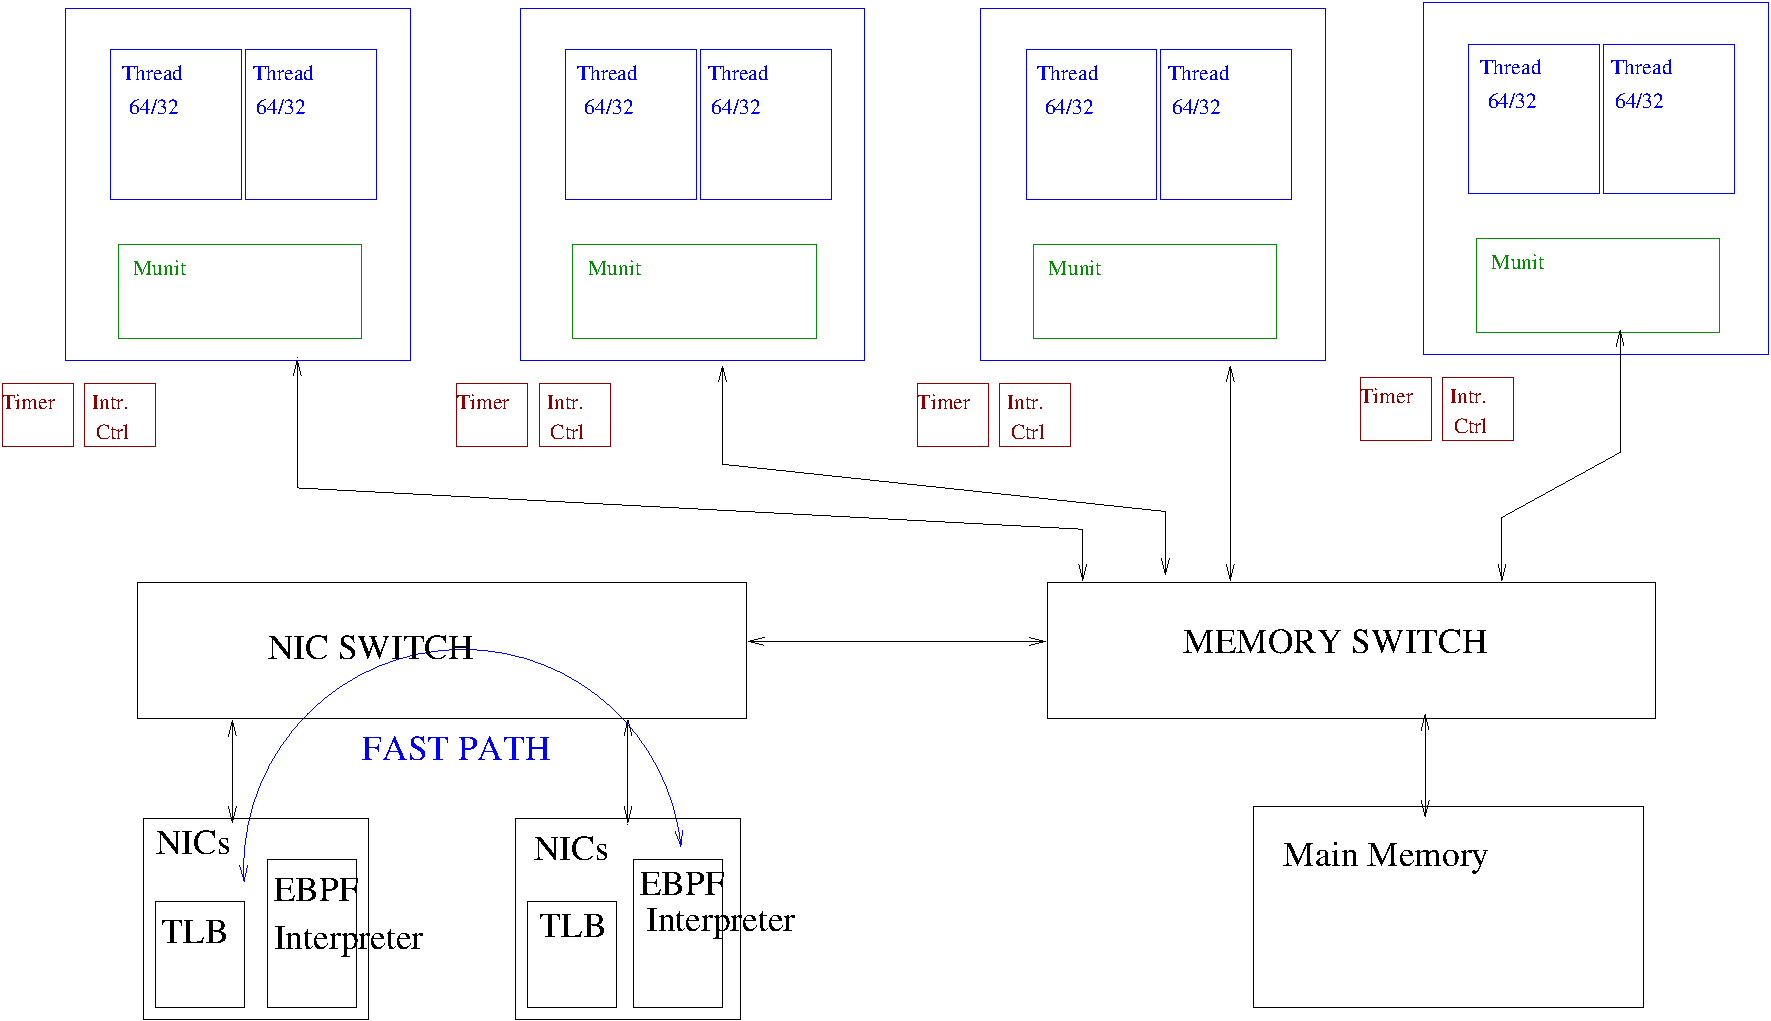
\includegraphics[width=10cm]{figs/Router_III.pdf}
  \caption{Router platform: phase 3}
\end{figure}
}

\frame[containsverbatim]{\frametitle{Comments on the proposed platform: Phase 3}
\begin{itemize}
\item NICs with lookup caches and embedded EBPF interpreter.
\begin{itemize}
\item NIC and main memory communicate directly.
\item NIC to NIC high performance direct paths are provided via
separate switch.
\item Packet processing in NIC using EBPF interpreter.
\item On lookup cache or interpreter hit, NIC to NIC packet
movement.
\end{itemize}
\item Processor cores handle remaining route lookups.
\end{itemize}
}

\frame[containsverbatim]{\frametitle{Development plan}
\begin{itemize}
\item Phase 1 (6 months):  port forwarding engine to 4-core 8-thread platform with vanilla NICs.
\item Phase 2 (6 months):  Control plane software port, add TLBs to NICs.
\item Phase 3 (6 months):  MPLS software port, add BPF interpreter to NICs.
\item On FPGA platform, demonstrate 1.6Gbps on Stage 1, 8 Gbps on Stage 2, 16 Gbps on Stage 3.
\item Seek funding to implement router ASIC (22nm, 1.2GHz, 10W).  Implementation will take 6-9 months.
\begin{itemize}
\item Target 100-200 Gbps in ASIC based router.
\end{itemize}
\end{itemize}
}

\frame[containsverbatim]{\frametitle{Scaling beyond quad-core}
\begin{figure}
  \centering
  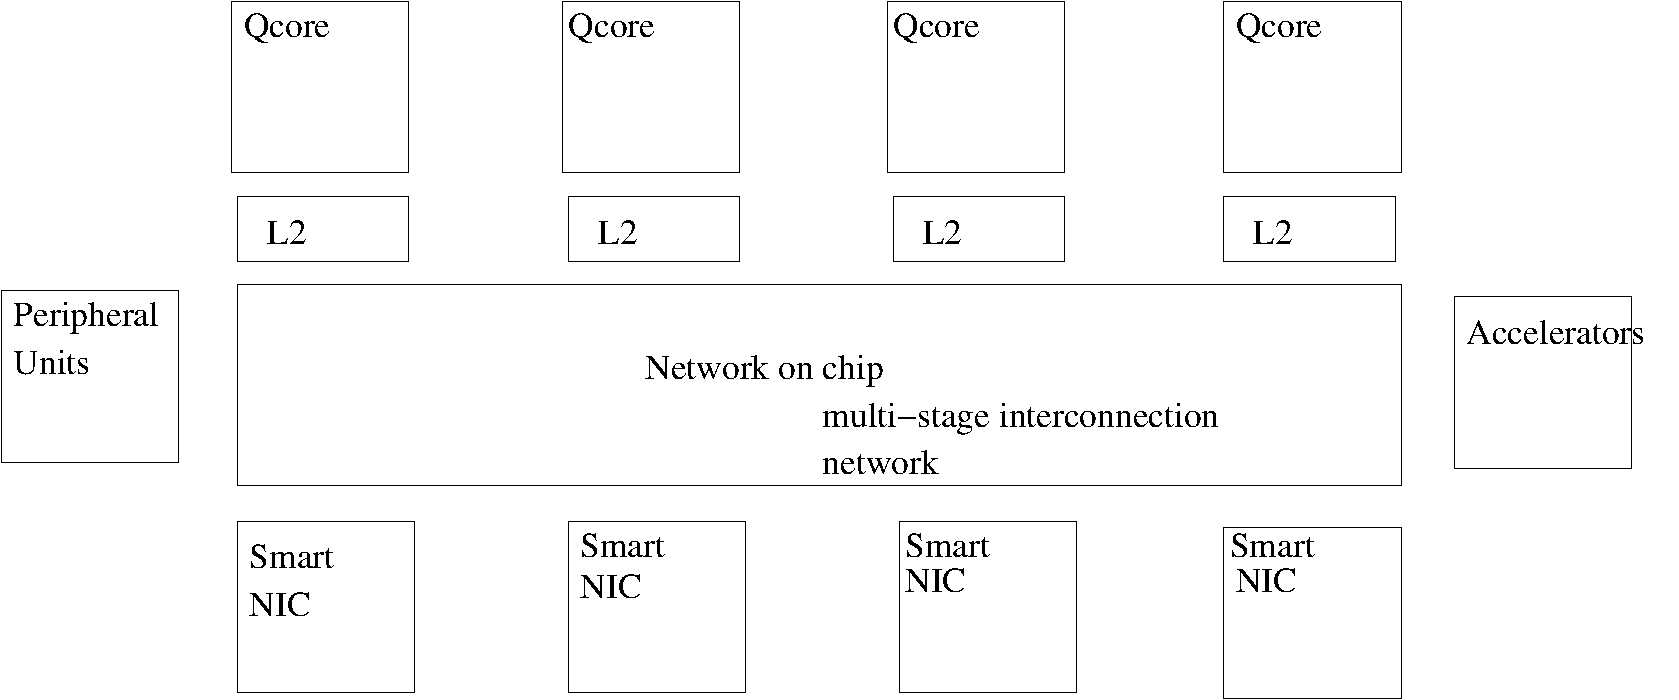
\includegraphics[width=10cm]{figs/Clusters.pdf}
  \caption{Clusters: scaling beyond quad-core}
\end{figure}
}

\frame[containsverbatim]{\frametitle{Comments on scaling beyond quad-core}
\begin{itemize}
\item Clusters of quad-cores (up to 256 quad-cores).
\item Each quad-core is internally cache coherent.
\item No cache coherence across quad-cores.
\item Communication between clusters based on message passing over internal
network.
\item Peripheral units TBD.
\item Accelerators TBD.
\item Network architecture TBD. 
\item Software programming environment: cooperative RTOS, TBD.
\end{itemize}
}

\end{document}

